\section{双曲线}
\subsection{双曲线的概念}
%@see: 《平面解析几何(甲种本)》 P91
平面内与两定点的距离的差的绝对值是常数(该常数小于两定点的距离)的点的集合
叫做\DefineConcept{双曲线}(hyperbola).
这两个定点叫做双曲线的\DefineConcept{焦点},
两焦点的距离叫做\DefineConcept{焦距}.

\subsection{双曲线的标准方程}
%@see: 《平面解析几何(甲种本)》 P92
取过焦点\(F_1\)和\(F_2\)的直线为\(x\)轴,
线段\(F_1 F_2\)的垂直平分线为\(y\)轴,
建立平面直角坐标系.

设\(P(x,y)\)是双曲线上的任意一点,双曲线的焦距是\(2c\ (c>0)\),
那么\(F_1\)和\(F_2\)的坐标分别是\((-c,0)\)和\((c,0)\).
又设点\(P\)与\(F_1\)和\(F_2\)的距离的差的绝对值等于正常数\(2a\).

由定义可知,双曲线就是点集\begin{equation*}
	\Set{ P \given \abs{\LineSegmentLength{P F_1} - \LineSegmentLength{P F_2}} = 2a }.
\end{equation*}
由两点间的距离公式,\begin{equation*}
	\LineSegmentLength{P F_1} = \sqrt{(x+c)^2+y^2},
	\qquad
	\LineSegmentLength{P F_2} = \sqrt{(x-c)^2+y^2},
\end{equation*}
将\(\LineSegmentLength{P F_1},\LineSegmentLength{P F_2}\)
代入\(\abs{\LineSegmentLength{P F_1} - \LineSegmentLength{P F_2}} = 2a\)
得\begin{equation*}
	\abs{\sqrt{(x+c)^2+y^2} - \sqrt{(x-c)^2+y^2}} = 2a,
\end{equation*}
化简,得\begin{equation*}
	(c^2-a^2) x^2 - a^2 y^2 = a^2 (c^2-a^2).
\end{equation*}
由双曲线的定义,\(
	2c > 2a,
	c > a,
	c^2 - a^2 > 0
\).
设\(b^2 = c^2 - a^2\ (b > 0)\),
代入上式得\begin{equation*}
	b^2 x^2 - a^2 y^2 = a^2 b^2,
\end{equation*}
也就是\begin{equation}\label{equation:平面解析几何.双曲线的标准方程1}
	\frac{x^2}{a^2} - \frac{y^2}{b^2} = 1.
\end{equation}
方程 \labelcref{equation:平面解析几何.双曲线的标准方程1} 叫做\DefineConcept{双曲线的标准方程},
它所表示的双曲线的焦点在\(x\)轴上,
它的焦点是\(F_1(-c,0)\)和\(F_2(c,0)\).

如果双曲线的焦点在\(y\)轴上,焦点是\(F_1(0,-c)\)和\(F_2(0,c)\),
那么只要将上面这个方程中的\(x\)、\(y\)互换,
就可以得到它的方程\begin{equation}\label{equation:平面解析几何.双曲线的标准方程2}
	\frac{y^2}{a^2}-\frac{x^2}{b^2}=1.
\end{equation}
方程 \labelcref{equation:平面解析几何.双曲线的标准方程2} 也是双曲线的标准方程.

\begin{figure}[htb]
	\centering
	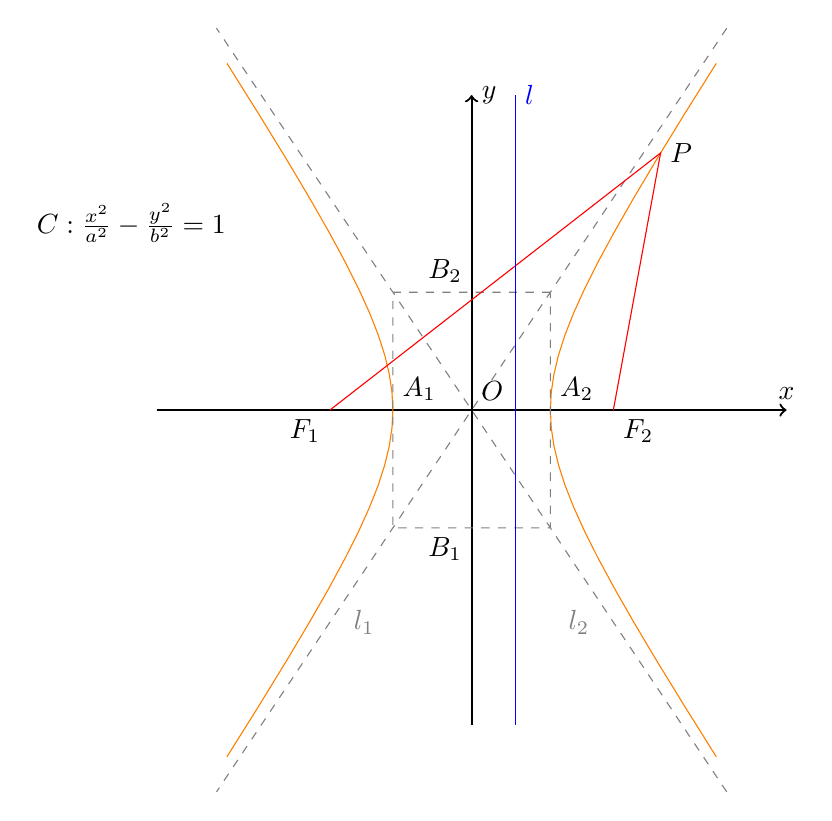
\begin{tikzpicture}
		%\draw[gray,help lines,dashed] (-5,-3) grid (5,3);
		\draw[thick,->] (-4,0) -- (4,0)node[above]{\(x\)};
		\draw[thick,->] (0,-4) -- (0,4)node[right]{\(y\)};
		\draw (-3,2)node[above left]{\(C: \frac{x^2}{a^2}-\frac{y^2}{b^2}=1\)};
		\pgfmathsetmacro{\e}{1.8}   % eccentricity
		\pgfmathsetmacro{\a}{1}
		\pgfmathsetmacro{\b}{(\a*sqrt((\e)^2-1)}
		\pgfmathsetmacro{\c}{(sqrt((\a)^2+(\b)^2))}
		\pgfmathsetmacro{\px}{2.4}
		\pgfmathsetmacro{\py}{sqrt(\b^2*(\px^2/\a^2-1))}
		\pgfmathsetmacro{\d}{1.8} % 定义域
		\draw[orange] plot[domain=-\d:\d] ({\a*cosh(\x)},{\b*sinh(\x)});
		\draw[orange] plot[domain=-\d:\d] ({-\a*cosh(\x)},{\b*sinh(\x)});
		\pgfmathsetmacro{\k}{1.8*\d}
		\coordinate (F1) at (-\c,0);
		\coordinate (F2) at (\c,0);
		\coordinate (P) at (\px,\py);
		\draw[gray,dashed] (\a,\b) -- (-\a,\b) -- (-\a,-\b) -- (\a,-\b) -- (\a,\b)
			(\k*\a,\k*\b) -- (-\k*\a,-\k*\b)
			(\k*\a,-\k*\b) -- (-\k*\a,\k*\b)
			(-\k*\a/2,-\k*\b/2)node[below right]{\(l_1\)}
			(\k*\a/2,-\k*\b/2)node[below left]{\(l_2\)};
		\draw[red] (F1)node[below left,black]{\(F_1\)}
			-- (P)node[right,black]{\(P\)}
			-- (F2)node[below right,black]{\(F_2\)};
		\pgfmathsetmacro{\dx}{\a^2/\c}
		\draw[blue] (\dx,-4) -- (\dx,4)node[right]{\(l\)}; % 准线
		\draw (0,0)node[above right]{\(O\)}
			(-\a,0)node[above right]{\(A_1\)}
			(\a,0)node[above right]{\(A_2\)}
			(0,-\b)node[below left]{\(B_1\)}
			(0,\b)node[above left]{\(B_2\)};
	\end{tikzpicture}
	\caption{双曲线的图形}
	\label{figure:平面解析几何.双曲线的图形}
\end{figure}

\subsection{双曲线的几何性质}
%@see: 《平面解析几何(甲种本)》 P94
我们根据双曲线的标准方程\begin{equation*}
	\frac{x^2}{a^2} - \frac{y^2}{b^2} = 1
\end{equation*}
来研究它的几何性质.
\begin{enumerate}
	\item 范围.

	由标准方程可知,双曲线上的点的坐标\((x,y)\)都适合不等式\(\frac{x^2}{a^2}\geq1\),
	即\(x^2 \geq a^2\),所以\(x \geq a\)或\(x \leq -a\).
	这说明双曲线在两条直线\(x = \pm a\)的外侧.

	\item 对称性.

	双曲线关于每条坐标轴和原点都是对称的.
	这时,坐标轴是双曲线的对称轴,原点是双曲线的对称中心.
	双曲线的对称中心叫做双曲线的\DefineConcept{中心}.

	\item 顶点.

	在标准方程中,令\(y=0\),得\(x = \pm a\),因此双曲线和\(x\)轴有两个交点\(A_1(-a,0)\)、\(A_2(a,0)\).因为\(x\)轴是双曲线的对称轴,所以双曲线和它的对称轴有两个焦点,它们叫做双曲线的\DefineConcept{顶点}.

	令\(x=0\),得\(y^2=-b^2\),这个方程没有实数根,说明双曲线和\(y\)轴没有交点,但我们也把\(B_1(0,-b)\)和\(B_2(0,b)\)画在\(y\)轴上.

	线段\(A_1 A_2\)叫做双曲线的\DefineConcept{实轴},它的长等于\(2a\),\(a\)叫做双曲线的实半轴长.
	线段\(B_1 B_2\)叫做双曲线的\DefineConcept{虚轴},它的长等于\(2b\),\(b\)叫做双曲线的虚半轴长.

	\item 渐近线.

	经过\(A_2\)、\(A_1\)作\(y\)轴的平行线\(x = \pm a\),
	经过\(B_2\)、\(B_1\)作\(x\)轴的平行线\(y = \pm b\),
	四条直线围成一个矩形.矩形的两条对角线所在的直线是\begin{equation*}
		y = \pm\frac{b}{a}x.
	\end{equation*}
	可以看出,双曲线的各支向外延伸时,与这两条直线逐渐接近.

	下面来证明上述事实.
	双曲线在第一象限内的部分的方程可以写为\begin{equation*}
		y = \frac{b}{a} \sqrt{x^2-a^2},
		\quad x > a.
	\end{equation*}
	设\(M(x,y)\)是这部分曲线上的点,
	\(N(x,z)\)是直线\(y = \frac{b}{a} x\)上与\(M\)有相同横坐标的点,
	即\(z = \frac{b}{a} x\).
	因为\begin{equation*}
		y = \frac{b}{a} \sqrt{x^2-a^2}
		= \frac{b}{a} x \sqrt{1 - \left( \frac{a}{x} \right)^2}
		< \frac{b}{a} x
		= z,
	\end{equation*}
	所以\begin{align*}
		\LineSegmentLength{MN}
		&= \abs{z - y}
		= z - y
		= \frac{b}{a} (x - \sqrt{x^2 - a^2}) \\
		&= \frac{b}{a}
			~ \frac{
				(x - \sqrt{x^2 - a^2})(x + \sqrt{x^2 - a^2})
			}{
				x + \sqrt{x^2 - a^2}
			} \\
		&= \frac{a b}{x + \sqrt{x^2 - a^2}}.
	\end{align*}
	过点\(M\)作垂线交直线\(y = \frac{b}{a} x\)于点\(Q\),
	\(\LineSegmentLength{MQ}\)就是点\(M\)到直线\(y = \frac{b}{a} x\)的距离.
	在直角三角形中,直角边边长小于斜边边长,
	所以\(\LineSegmentLength{MQ} < \LineSegmentLength{MN}\).
	当\(x\)逐渐增大时,
	\(\LineSegmentLength{MN}\)逐渐减小.
	当\(x\)充分大时,
	\(\LineSegmentLength{MN}\)就充分接近于零,
	从而\(\LineSegmentLength{MQ}\)也充分接近于零.
	这就说明双曲线在第一象限的部分从射线\(ON\)的下方逐渐接近于射线\(ON\).

	在其他象限内也可以证明类似的情况.
	我们把这两条直线叫做双曲线的\DefineConcept{渐近线}.

	在方程\(\frac{x^2}{a^2}-\frac{y^2}{b^2}=1\)中,
	如果\(a=b\),那么双曲线方程为\(x^2-y^2=a^2\),
	它的实轴和虚轴的长都等于\(2a\).
	这时,四条直线\(x=\pm a\)、\(y=\pm a\)围成正方形;
	渐近线方程成为\(x=\pm y\),它们互相垂直,并且平分双曲线实轴与虚轴所成的角.
	像这样,实轴和虚轴等长的双曲线叫做\DefineConcept{等轴双曲线}.

	\item 离心率.

	双曲线的焦距与实轴的比\(e = \frac{c}{a}\),
	叫做双曲线的\DefineConcept{离心率}.

	因为\(c > a\),所以双曲线的离心率\(e > 1\).

	由等式\(c^2-a^2=b^2\)可得\begin{equation*}
		\frac{b}{a} = \frac{\sqrt{c^2-b^2}}{a}
		= \sqrt{\frac{c^2}{a^2}-1} = \sqrt{e^2-1}.
	\end{equation*}
	因此\(e\)越大,\(\frac{b}{a}\)也越大,
	即渐近线\(y = \pm\frac{b}{a}x\)的斜率的绝对值越大,
	这时双曲线的形状就从褊狭逐渐变得开阔.
	由此可知,双曲线的离心率越大,它的开口就越开阔.
\end{enumerate}

\begin{example}
%@see: 《平面解析几何(甲种本)》 P98 例3
以已知双曲线的虚轴为实轴,实轴为虚轴的双曲线叫做原双曲线的\DefineConcept{共轭双曲线}.
求证:\begin{enumerate}
	\item 双曲线和它的共轭双曲线有共同的渐近线;
	\item 双曲线和它的共轭双曲线的四个焦点在同一个圆上.
\end{enumerate}
\begin{proof}
设已知双曲线的方程是\begin{equation*}
	\frac{x^2}{a^2}-\frac{y^2}{b^2}=1.
\end{equation*}
它的焦点坐标为\(F_1(-c,0)\)和\(F_2(c,0)\)
(\(c^2=a^2+b^2\)).
它的渐近线方程是\(y=\pm\frac{b}{a}x\).

根据定义,其共轭双曲线的方程是\begin{equation*}
	\frac{y^2}{a^2}-\frac{x^2}{b^2}=1.
\end{equation*}
它的交点坐标为\(F'_1(0,-c)\)和\(F'_2(0,c)\),
可见四个焦点都在圆\(x^2+y^2=c^2\)上.
它的共轭双曲线的渐近线方程是\(x=\pm\frac{a}{b}y\),
也即\(y=\pm\frac{b}{a}x\),
所以双曲线和它的共轭双曲线具有共同的渐近线.
\end{proof}
\end{example}

\begin{example}
%@see: 《平面解析几何(甲种本)》 P99 例4
点\(P(x,y)\)与定点\(F(c,0)\)的距离
和它到定直线\(l: x = \frac{a^2}{c}\)的距离的比是
常数\(\frac{c}{a}\ (c > a > 0)\).
求点\(P\)的轨迹.
\begin{solution}
设点\(P\)到直线\(l\)的距离是\(d\),那么所求轨迹就是点集\begin{equation*}
	\Set*{ P \given \frac{\LineSegmentLength{PF}}{d} = \frac{c}{a} },
\end{equation*}
由此得\begin{equation*}
	\frac{\sqrt{(x-c)^2+y^2}}{\abs{\frac{a^2}{c}-x}} = \frac{c}{a},
\end{equation*}
化简得\begin{equation*}
	(c^2-a^2)x^2 - a^2 y^2 = a^2(c^2-a^2).
\end{equation*}
设\(b^2=c^2-a^2\),则可将上式进一步化简为\begin{equation*}
	\frac{x^2}{a^2}-\frac{y^2}{b^2}=1.
\end{equation*}
这是双曲线的标准方程,所以点\(P\)的轨迹是双曲线.
\end{solution}
\begin{remark}
由上例可知,点\(P\)与一个定点的距离和它到一条定直线的距离的比是常数
\(e = \frac{c}{a} > 1\)时,
这个点的轨迹是双曲线.
定点是双曲线的焦点,定直线叫做双曲线的\DefineConcept{准线},
常数\(e\)是双曲线的离心率.
\end{remark}

对于双曲线\(\frac{x^2}{a^2}-\frac{y^2}{b^2}=1\),
相应于焦点\(F(c,0)\)的准线方程是\begin{equation*}
	x = \frac{a^2}{c}
	\quad\text{或}\quad
	x = \frac{a}{e}.
\end{equation*}
根据双曲线的对称性,
相应于焦点\(F'(-c,0)\)的准线方程是\(x=-\frac{a^2}{c}\),
所以双曲线有两条准线.
\end{example}

\begin{example}
%@see: 《平面解析几何(甲种本)》 P102 习题七 9.
证明:等轴双曲线的离心率是\(\sqrt2\).
\begin{proof}
由定义,等轴双曲线\(x^2-y^2=a^2\)的实半轴长与虚半轴长相等,
即\(a=b>0\),
故\(c^2 = a^2 + b^2 = 2 a^2\),
\(c = \sqrt2 a\),
那么等轴双曲线的离心率为\begin{equation*}
	e = \frac{c}{a} = \frac{\sqrt2 a}{a} = \sqrt2.
	\qedhere
\end{equation*}
\end{proof}
\end{example}

\begin{example}
%@see: 《平面解析几何(甲种本)》 P102 习题七 12.
证明:从双曲线的一个焦点到一条渐近线的距离等于虚半轴长.
\begin{proof}
设双曲线方程为\begin{equation*}
	\frac{x^2}{a^2}-\frac{y^2}{b^2}=1,
\end{equation*}
它的右焦点为\(F(c,0)\)
(\(c^2=a^2+b^2\)),
其中一条渐近线为\(y=\frac{b}{a}x\)或\(bx-ay=0\).
由点到直线的距离公式,焦点\(F\)到上述渐近线的距离为\begin{equation*}
	d = \frac{\abs{b \cdot c - a \cdot 0}}{\sqrt{b^2+(-a)^2}}
	= \frac{bc}{c} = b.
	\qedhere
\end{equation*}
\end{proof}
\end{example}

\begin{example}
已知双曲线\begin{equation*}
	C: \frac{x^2}{a^2} - \frac{y^2}{b^2} = 1
	\quad(a>b>1).
\end{equation*}
求双曲线在其上任意一点\(P_0(x_0,y_0)\)处的切线方程.
\begin{solution}
因为点\(P_0(x_0,y_0)\)在双曲线\(C\)上,
所以\begin{equation*}
	\frac{x_0^2}{a^2} - \frac{y_0^2}{b^2} = 1
	\quad\text{即}\quad
	b^2 x_0^2 - a^2 y_0^2 = a^2 b^2.
\end{equation*}

当切线\(l\)与\(x\)轴相垂直时,
显然只有\((-a,0)\)和\((a,0)\)两点可能是切点,
而它们各自的切线方程分别为\(x=-a\)和\(x=a\).

当切线\(l\)不与\(x\)轴相垂直时,
设切线方程为\(l: y = kx + p\),
其中\(p = y_0 - k x_0\).
联立方程组,
得\begin{equation*}
	\begin{cases}
		y = kx + p, \\
		\frac{x^2}{a^2} - \frac{y^2}{b^2} = 1.
	\end{cases}
\end{equation*}
那么有\begin{gather*}
	\frac{1}{a^2} x^2 - \frac{1}{b^2} (kx+p)^2 = 1, \\
	b^2 x^2 - a^2 (k^2 x^2 + 2kpx + p^2) = a^2 b^2, \\
	(b^2 - a^2 k^2) x^2 - 2 a^2 k p x - a^2 (p^2 + b^2) = 0.
\end{gather*}
令判别式\(\Delta_1 \defeq (2 a^2 k p)^2 + 4 (b^2 - a^2 k^2) a^2 (p^2 + b^2) = 0\),
得\begin{gather*}
	4 a^4 k^2 p^2 = 4 (a^2 k^2 - b^2) a^2 (p^2 + b^2), \\
	a^2 k^2 p^2 = (a^2 k^2 - b^2)(p^2 + b^2), \\
	a^2 b^2 k^2 = b^2(p^2 + b^2), \\
	a^2 k^2 = p^2 + b^2,
\end{gather*}
代入\(p = y_0 - k x_0\),
得\begin{equation*}
	a^2 k^2 = (y_0 - k x_0)^2 + b^2, \\
	y_0^2 - 2k x_0 y_0 + k^2 x_0^2 + b^2 = a^2 k^2, \\
	(x_0^2 - a^2) k^2 - 2 x_0 y_0 k + (y_0^2 + b^2) = 0.
\end{equation*}
上式的判别式\(
	\Delta_2
	\defeq (2 x_0 y_0)^2 - 4(x_0^2 - a^2)(y_0^2 + b^2)
	= 4(a^2 b^2 + a^2 y_0^2 - b^2 x_0^2)
	= 0
\),
故可解得\begin{equation*}
	k = \frac{2 x_0 y_0}{2 (x_0^2 - a^2)}
	= \frac{x_0 y_0}{x_0^2 - a^2}.
\end{equation*}
那么\(l\)的方程为\begin{gather*}
	y - y_0 = \frac{x_0 y_0}{x_0^2 - a^2} (x - x_0), \\
	(x_0^2 - a^2) y = x_0 y_0 x + (x_0^2 - a^2) y_0 - x_0^2 y_0
	= x_0 y_0 x - a^2 y_0, \\
	x_0 y_0 x + (a^2 - x_0^2) y = a^2 y_0, \\
	\frac{x_0 x}{a^2} + (a^2 - x_0^2) \frac{y_0 y}{a^2 y_0^2} = 1, \\
	\frac{x_0 x}{a^2} + (a^2 - x_0^2) \frac{y_0 y}{(x_0^2 - a^2) b^2} = 1,
\end{gather*}
最后化简得\begin{equation}\label{equation:平面解析几何.双曲线的切线}
	\frac{x_0 x}{a^2} - \frac{y_0 y}{b^2} = 1.
\end{equation}
这就是双曲线在其上任意一点\(P_0(x_0,y_0)\)处的切线方程.
\end{solution}
\end{example}

\begin{theorem}[双曲线的焦点三角形]
设\(P\)是双曲线\(C: \frac{x^2}{a^2} - \frac{y^2}{b^2} = 1\ (a>0,b>0)\)上任一点,
\(F_1\)和\(F_2\)是\(C\)的焦点,那么\begin{equation*}
	S_{\triangle P F_1 F_2} = \frac{b^2}{\tan(\theta/2)},
\end{equation*}
其中\(\theta=\angle{F_1 P F_2}\).
%TODO proof
\end{theorem}
